
\chapter{人机交互式机器翻译系统设计与实现}
\label{Chapter_implementation}

我们在第二章综述中介绍了人机交互式机器翻译技术,但目前市场上尚无公开可用的人机交互式机器翻译系统。无论是谷歌等在线机器翻译,还是Systran、Moses、NiuTrans等可定制的机器翻译,一般都还局限于纯粹的机器翻译系统。而商业化的Trados、MemoQ等计算机辅助翻译软件往往通过插件的方式直接调用第三方机器翻译的最终结果,与机器翻译无实质的人机交互过程。因此,在本章中,基于第三到第五章的人机交互式机器翻译技术,我们尝试设计和实现可用于人工翻译场景中的人机交互式英汉机器翻译系统。

如前文所述,人机交互式机器翻译正处于走向实用化的关键时期,在未来仍然主要面对三方面的问题:用户如何更高效地使用机器翻译;机器翻译如何利用已有的外部资源提高自动译文质量以减少用户的重复劳动;机器翻译如何根据用户上下文进行自适应以完成模型和参数的自动更新。这三个问题是本论文致力于解决的问题,也是本章设计与实现的系统要解决的问题。

\section{基本思想}

人机交互式机器翻译系统的基本思想是,在同一套系统里实现机器翻译和计算机辅助翻译功能的归一化,使得系统有良好的人机交互体验,能够方便地进行人工翻译作业,从而提高人工翻译效率。

在人机交互式机器翻译系统中,主要功能模块被划分成四种类型:语料管理模块、状态管理模块、解码器管理模块和模型管理模块。

语料管理模块的作用是管理术语库和翻译记忆库,主要功能包括导入导出外部数据文件、快速检索等。

状态管理模块的作用是管理人工翻译项目,跟踪译员实时状态,收集人机交互所需要的上下文信息,主要功能包括导入导出翻译文档、生成和维护项目文档结构树、上下文信息缓存、译员状态跟踪、多用户协作等。其中,项目文档结构树指实时记录和管理项目文档的格式、句子翻译状态、译文版本等信息的数据结构。上下文信息包括当前句子对应机器翻译解码器的翻译规则和翻译假设等深层次信息,术语库和翻译记忆库的匹配状态等。译员状态包括当前光标位置、用户按键序列和鼠标点击序列等信息。状态管理模块是实现人机交互式机器翻译系统的关键模块,是各模块的实时状态数据交换中心,也是人机交互式机器翻译区别于传统机器翻译以及传统计算机辅助翻译系统的重要特征。

解码器管理模块的作用,除了管理机器翻译相关的解码器和解码器的各项参数,还包括分析和调用用户编写的机器翻译规则库等。本章中设计的解码器主要为人机交互服务,包括核心解码器和附属解码器。其中,附属解码器包括术语翻译解码器(“TB+解码器”)、翻译记忆解码器(“TM+解码器”)和命名实体解码器(“NE解码器”),分别负责与术语库、翻译记忆库和命名实体识别模块的信息进行融合解码。机器翻译核心解码器根据输入的源语言句子,综合各附属解码器的结果,生成并输出目标语言的自动译文。输入法核心解码器根据用户按键序列,综合状态管模块的信息,生成并输出输入法的输入结果和译文提示。另外,统计机器翻译的最小错误率训练也属于解码器管理模块的功能。

模型管理模块的作用是训练和管理语言模型、调序模型和翻译模型等模型,还包括这些模型的调用、数据的保存与加载等。

\section{系统设计}

人机交互式机器翻译系统的结构图如图\ref{Fig_system_overview}所示。本文设计的人机交互式机器翻译系统采用服务器/客户端架构。由于客户端的系统结构可参考通用软件设计,且较多涉及与本文无关的技术细节,因此本章仅讨论服务器端的系统结构。

从图\ref{Fig_system_overview}可以看出,整个系统可分为六层,从上至下分别为接口层、控制层、业务层、模型层、缓冲层和数据库。

最上层的接口层直接与客户端通信,接收客户端请求并返回调用结果。通信方式采用远程方法调用(remote method invocation,RMI)和Web Service。为增强系统鲁棒性,同时为系统安全考虑,接口层应用了反向代理(reverse proxy)技术。

控制层管理和控制接口层的功能调用,同时确保上层的调用请求被成功转发到业务层,具体功能包括处理异常、恢复错误、监控系统状态、记录访问日志、均衡负载和部署代码等。如果系统需要对用户的操作权限进行管理,则权限控制的功能也隶属于控制层。

业务层实现人机交互式机器翻译的主要业务逻辑,是接口层对外提供功能的实际执行者,包括语料管理模块、状态管理模块和解码器管理模块。业务层功能还包括系统管理、数据迁移等面向系统管理员的功能。

模型层为业务层的解码器提供模型支持,包括各模型的管理和训练模块,以及各模型依赖的基础组件,如词汇表、大小写转换、分词模块、命名实体识别模块等。模型层的主要功能是从数据库和缓冲层中加载数据,并将热点数据放入缓存中。

缓冲层为整个系统提供数据缓存支持,本文中用到的技术包括 Hibernate、 Ehcache 和 Memcached, 可以为不同类型的模型数据提供不同的缓存策略。

最底层为数据库,为整个系统的数据提供持久化支持。本文使用MySQL数据库,在有分布式需求时,可以顺利完成主从复制和读写分离。

\begin{figure}[!tb]
	\centering
	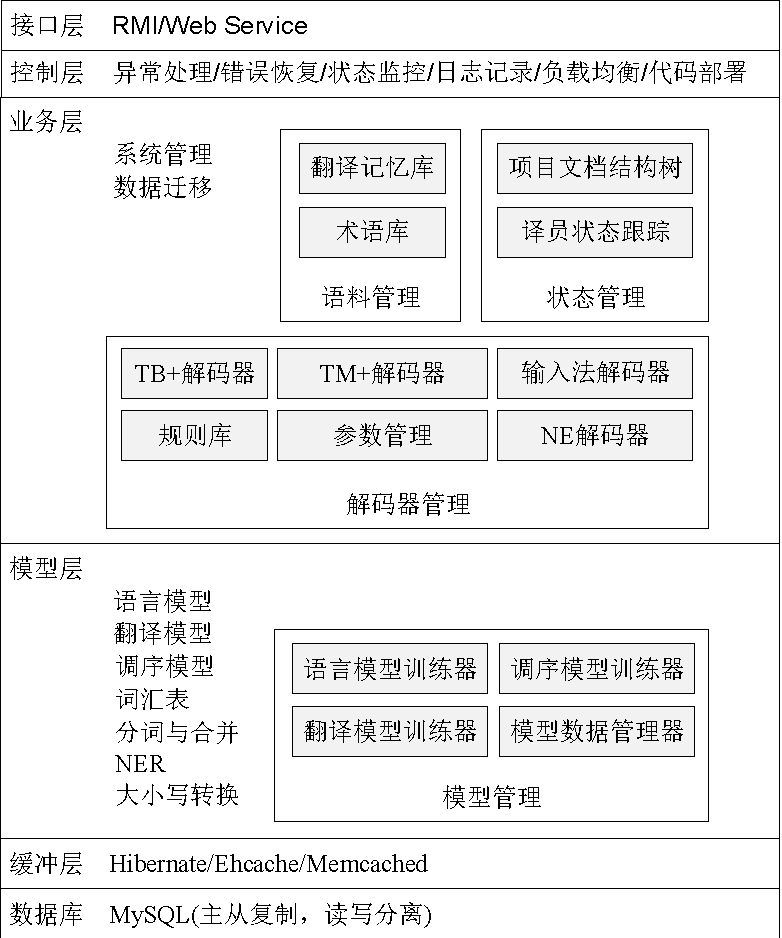
\includegraphics[width=0.9\textwidth]{Figure/Figure_6_1.pdf}
	\caption{人机交互式机器翻译系统结构图}
	\label{Fig_system_overview}
\end{figure}

\section{系统实现}

在本文中,人机交互式机器翻译系统的整体架构采用服务器/客户端模式。我们采用Apache Flex作为客户端的编程语言,使用Adobe Flash Catalyst作为图形界面设计工具,采用Java作为服务器端的主要编程语言。限于篇幅,功能实现的具体细节不再赘述,我们以CoCat输入法为例说明功能实现过程中遇到的挑战和应对方案。

\begin{figure}[!tb]
	\centering
	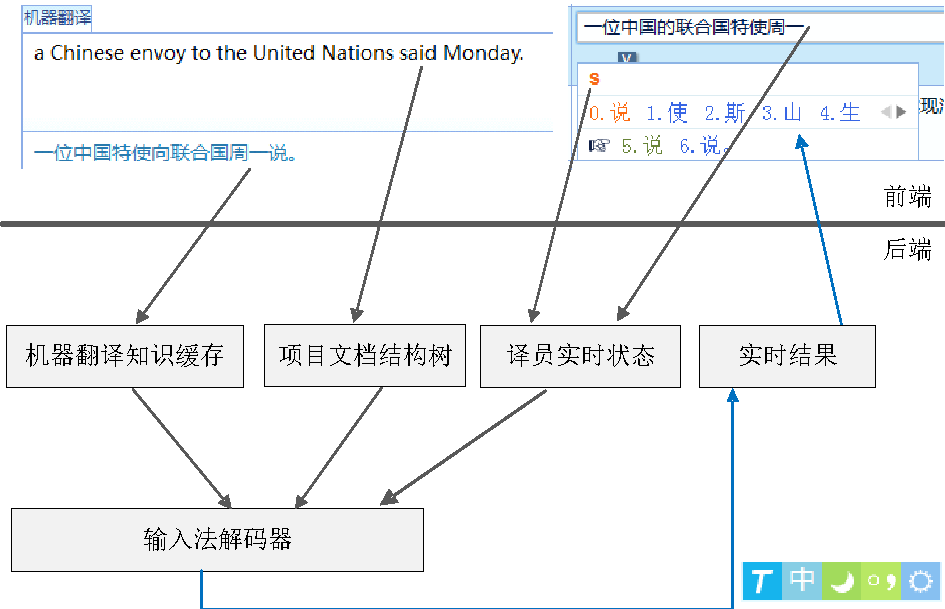
\includegraphics[width=0.9\textwidth]{Figure/Figure_6_2.pdf}
	\caption{CoCat输入法异步通信原理图}
	\label{Fig_system_communication}
\end{figure}

图\ref{Fig_system_communication}给出了CoCat输入法的实现原理图。译员在翻译源语言句子“a Chinese envoy to the United Nations Said Monday.”时,机器翻译给出的自动译文为“一位中国特使向联合国周一说。”很显然,机器翻译自动译文不能直接使用。译员使用CoCat输入法开始翻译。图\ref{Fig_system_communication}给出了译员在前端的图形界面已输入“一位中国的联合国特使”后再按键“s”时的系统瞬间。在这个瞬间,后端的项目文档结构树子模块记录了当前正在翻译的源语言句子和译员已录入的部分目标译文,译员状态跟踪子模块记录了当前的光标位置和键盘按键序列,上下文信息子模块缓存了机器翻译系统为翻译该句子加载的翻译规则、翻译假设和n-best列表等机器翻译知识,以及术语库和翻译记忆库实时检索状态信息等。此时,后端的输入法解码器需要根据机器翻译知识缓存、项目文档结构树和译员实时状态快速对按键序列解码,并将输入法的实时结果推送到前端的图形界面。从译员按下“s”键到他看见输入法短语候选,时间不能长于0.2秒,否则用户会感觉到系统的卡顿。

需要注意的是,在输入法解码器计算期间,用户可能改变了已有的按键序列,比如删除了“s”或者增加了“h”。此时,输入法解码器应该停止当前的计算过程,并立即开始新一轮解码,尽量不能让用户感觉到输入法卡顿。但技术实现的难度非常大。CoCat输入法需要用到机器翻译知识缓存和项目文档结构树,因此只能在服务器端执行输入法解码过程。这除了要求输入法解码器本身的解码算法足够快,整个链路的通信也必须保持极低的延时。相对而言,仅提供API服务的机器翻译系统并不一定需要提供复杂的交互功能和保证低延时。

为了实现良好的人机交互体验,我们将同步的前后端通信方式调整为异步通信。即调整前,前端以按键序列等作为参数调用后端的输入法API,然后等待输入法API返回计算结果,并将结果显示在图形界面上,当按键序列更新时,重复这个过程。同步通信的主要问题是当用户同时按键时,上一个请求还未返回结果时,新的请求就已发出。如果两次请求间隔非常短或者网络发生不规律的延迟,就可能出现后发请求却先接收到响应,然后再被过期的响应覆盖,图形界面上最后显示的是过期的结果。而将通信方式调整为异步通信之后,前端提交按键序列后直接返回,当按键序列更新时,继续提交。服务器端接收到新的按键序列,立即停止该用户未完成的解码过程,然后开始新的解码过程,然后将实时结果提交给同步线程。在异步通信方式下,同步线程一直检测是否有结果需要推送到前端,而前端一直等待接收服务器后端的推送信息。

这样,虽然如图\ref{Fig_system_communication}异步通信仍然可能会因为推送过程的意外延迟而出现的卡顿,但前端出现卡顿的概率大幅下降,用户交互体验得到显著改善。当大量用户连接同一台服务器时,异步通信的优势则更为明显。在实现人机交互式机器翻译系统过程中,类似的改进还有很多。由于篇幅限制,不再赘述。

\begin{figure}[!bt]
	\centering
	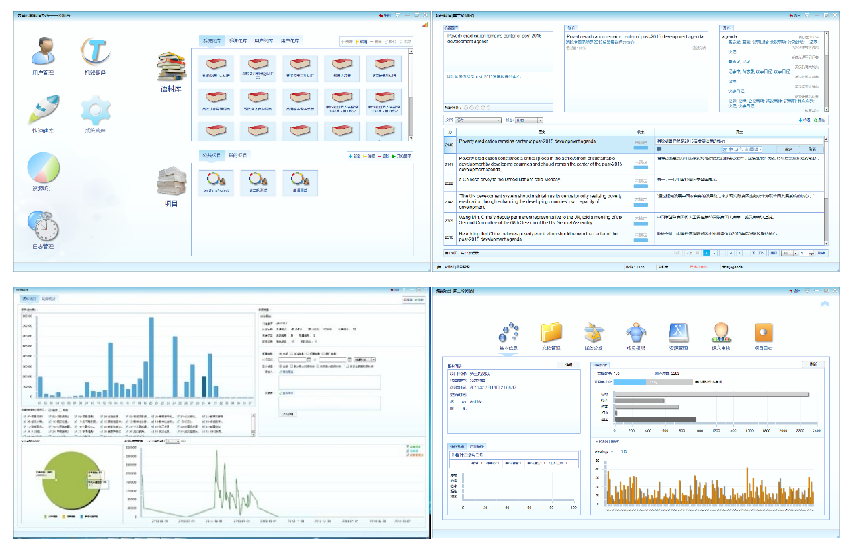
\includegraphics[width=\textwidth]{Figure/Figure_6_3.pdf}
	\caption{人机交互式翻译系统前端图形界面}
	\label{Fig_system_gui}
\end{figure}

在本文中实现的人机交互式机器翻译系统图形界面如图\ref{Fig_system_gui}所示。由于图形界面不是本文关注的重点,也不再赘述。

\section{经验总结}

在人机交互式机器翻译系统实现过程中,我们认为下列经验也许可以为未来的相关工作提供借鉴:

(1)对于人机交互式机器翻译系统开发任务而言,最重要的是要明确用户的具体需求;

(2)人机交互式机器翻译系统的要义在交互,因此需要加强自动译文的可控性和系统的在线自适应能力;

(3)为生产力工具的设计者和开发者,需要对编程语言、操作系统、网络通信、数据库、分布式架构等有全面的了解,尽量避免使用花哨和不可控的技术;

(4)对于人工翻译而言,一个实用功能远比自动译文一个BLEU百分点的提升受欢迎。

\section{本章小结}

在本章中,我们尝试设计和实现了用于人工翻译场景中的人机交互式英汉机器翻译系统。该系统的主要功能模块被划分成四种类型:语料管理模块、状态管理模块、解码器管理模块和模型管理模块。结构方面,整个系统可分为六层:接口层、控制层、业务层、模型层、缓冲层和数据库。然后以CoCat输入法为例,介绍了系统实现。最后总结了系统实现过程中的一些经验。